%%%%%%%%%%%%%%%%%%%%%%%
\documentclass[english,  % Standardmäßig deutsche Eigenarten, englisch -> english
parskip=full,  % Absätze durch Leerzeile trennen 
%%%%%%%%%%%%%%%%%%%%%%%
%bibliography=totoc,  % Literatur im Inhaltsverzeichnis (ist unüblich)
%draft,  % TODO: Entwurfsmodus -> entfernen für endgültige Version
headsepline]{scrartcl}
\usepackage[utf8]{inputenc}  % Kodierung der Datei
\usepackage[T1]{fontenc}  % Vollen Umfang der Schriftzeichen
\usepackage[english]{babel}  % Sprache auf Deutsch (neue Rechtschreibung)
%%%%%%%%%%%%%%%%%
\usepackage[a4paper,left=3.5cm, right=3.5cm,top=3.5cm, bottom=5.7cm]{geometry}
%%%%%%%%%%%%%%%%%
\usepackage{layout}
\usepackage{booktabs}
\usepackage{float}
% Mathematik und Größen
\usepackage{amsmath}
\usepackage[locale=US,  % englische Eigenarten, deutsch -> DE
separate-uncertainty,  % Unsicherheiten seperat angeben (mit ±)
]{siunitx}
%http://texdoc.net/texmf-dist/doc/latex/siunitx/siunitx.pdf
\usepackage{physics}  % Erstellung von Gleichungen vereinfachen
\usepackage{svg}    
\usepackage{graphicx}  % Bilder einbinden \includegraphics{Pfad/zur/Datei(ohne Dateiendung)}
\usepackage[
backend=biber,
style=nature,
sorting=ynt
]{biblatex}
\usepackage{wrapfig}
\usepackage[version=4,arrows=pgf]{mhchem}  % Chemie Paket für Isotopenschreibweise etc.
\usepackage{wrapfig}
\usepackage{floatflt}
\usepackage{enumerate}
% Gestaltung
%\usepackage{microtype}  % Mikrotypographie (kann man am Ende verwenden)
\usepackage{booktabs}  % schönere Tabellen
%\usepackage[toc]{multitoc}  % mehrspaltiges Inhaltsverzeichnis
\usepackage{multicol}
\usepackage{csquotes}  % Anführungszeichen mit \enquote
\usepackage{caption}  % Anpassung der Bildunterschriften, Tabellenüberschriften
\usepackage{subcaption}  % Unterabbildungen, Untertabellen, …
\usepackage{cprotect}
\usepackage{enumitem}  % Listen anpassen
\usepackage{siunitx}
\usepackage{eufrak}
\usepackage{dirtytalk}
\usepackage{subcaption}
\usepackage{textcomp}
\usepackage{circuitikz}
\setlist{itemsep=-10pt}  % Abstände zwischen Listenpunkten verringern
\addbibresource{bibliography.bib}
% Manipulation des Seitenstils
\usepackage{scrlayer-scrpage}
% Kopf-/Fußzeilen setzen
\pagestyle{scrheadings}  % Stil für die Seite setzen
\clearscrheadings  % Stil zurücksetzen, um ihn neu zu definieren
\automark{section}  % Abschnittsnamen als Seitenbeschriftung verwenden
\ofoot{\pagemark}  % Seitenzahl außen in Fußzeile
\ihead{\headmark}  % Seitenbeschriftung mittig in Kopfzeile
%\setkomafont{\headsepline}{}
\setcounter{tocdepth}{2} %set depth of printed table of contets.

\makeatletter

%\renewcommand\tableofcontents{% Absatz vor Gliederungspunkten
   % \begin{multicols}{2}[\section*{\contentsname
 %       \@mkboth{%
  %         \MakeUppercase\contentsname}{\MakeUppercase\contentsname}}]%
 %   \@starttoc{toc}%
 %   \end{multicols}%
 %   }

\makeatother %print dots in sections in toc.

\usepackage[hidelinks]{hyperref}  % Links und weitere PDF-Features
\usepackage{hyperref}
\hypersetup{
    colorlinks=true,
    linkcolor=blue,
    citecolor=red,
    filecolor=magenta,      
    urlcolor=cyan,
    pdftitle={Overleaf Example},
    pdfpagemode=FullScreen,
    }
\usepackage[]{cleveref} %noabbrev für ausgeschriebene verweise
% TODO: Titel und Autor, … festlegen
\newcommand*{\titel}{Solar cell}
\newcommand*{\autor}{Lukas König, Steven Gebel}
\newcommand*{\abk}{}
\newcommand*{\betreuer}{Elizabeth Christine Baird}
\newcommand*{\messung}{25. November 2021}
\newcommand*{\ort}{KRO/Lab 2.15}
\newcommand{\diff}[1]{\frac{\mathrm{d}}{\mathrm{d}#1}}
\newcommand{\mum}{\:\si{\mu m\:}}
\newcommand{\ten}[1]{\cdot10^{#1}}
\newcommand{\dsys}{\Delta_\text{sys}}
\newcommand{\logdiff}[1]{\left(\frac{\Delta #1}{#1}\right)^2}
\newcommand{\dunderline}[1]{\underline{\underline{#1}}}
\newcommand{\bcref}[1]{\namecref{#1} \textcolor{blue}{\labelcref{#1}}}

\hypersetup{pdfauthor={\autor}, pdftitle={\titel}}  % PDF-Metadaten setzen

% automatischen Titel konfigurieren
\titlehead{Fortgeschrittenenpraktikum LM \abk \hfill Technische Universität Dresden}
\subject{Lab report}
\title{\titel}
\author{\autor}
\date{\begin{tabular}{ll}
Protocol: & \today\\
Measurement: & \messung\\
Place: & \ort\\
Supervisor: & \betreuer\end{tabular}}
\begin{document}
\begin{titlepage}
\maketitle  % Titel setzen
\tableofcontents  % Inhaltsverzeichnis setzen
\end{titlepage}
\section{Introduction}
\subsection{Task}
% übersetzen
\begin{itemize}
    \item A: Measure a dark and a light characteristic curve of an inorganic cell under the intensity of a sun
    \item B: Measure the I-V-characteristic curve of an inorganic cell at five different light intensities.
    \item C: Setup 6 inorganic cells so that the module works with as little loss as possible and with little failure. Subsequently record the characteristic curve.
    Connect series/parallel resistors outside the module in three combinations. Record the characteristic curve. Investigate the behaviour for partial shading of the module for three shading situations.
    Construct a bigger module, consisting of more solar cells, with output of at least $\SI{6}{\volt}$, record the characteristics. Connect a load and record the characteristic again. Determine the working voltage and current using a multimeter.
    \item D: Measure the temperature dependence of the open circuit voltage $V_{OC}$ of an individual inorganic cell from approx. $30\si{\celsius}$ to $65\si{\celsius}$. Measure the characteristic curve at the lowest and highest temperature.
   \item E: Compare the dependence of the short-circuit current $I_{SC}$ and the angle of incidence of light in 10° steps of an inorganic cell.
\end{itemize}
\subsection{Theoretical background}
\subsubsection{Basics}
A solar cell works through the photovoltaic effect, where photons are used to excite charge-carriers in a material. Three conditions have to be met to allow this:
\begin{enumerate}
    \item Radiation has to be absorbed
    \item The absorption has to lead to the excitation of negative and positive charge carriers and
    \item The charges have to be separated.
\end{enumerate}
1 and 2 are met by using semi-conductors, the third condition is achieved by a transition between different semiconductors.
\subsubsection{Semiconductors}
A metal is called a semiconductor if it has a resistivity between \SIrange{e-4}{e6}{\ohm m}. A further characteristic of semiconductors is that their conductivity rises with temperature.
\paragraph{Band-gap model}
To explain the properties of a semiconductor, the band-gap model is a useful tool. Bands form in condensed matter as a result of the superposition of the many electron-wavefunctions. The situation is depicted for different types of solid matter in \cref{fig:bandstructures}. The mean energy of the highest occupied state is called Fermi-energy $E_F$ In metals, the outer band is not completely filled, offering electrons free states to move to without a significant change in energy, leading to high conductivity. In semiconductors and isolators however, the valence-band (the highest band at 0\,K), is fully occupied at $T=0$\,K, thus leading to a band-gap and to the nonconductivity of those materials. Semiconductors and isolators are only differentiated by the width of the band-gap $E_G$ ($<3$eV in semiconductors).
\begin{figure}[H]
    \centering
    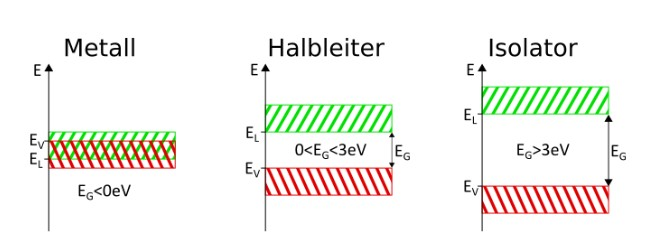
\includegraphics[width=0.7\linewidth]{bandstructures.jpg}
    \caption{Bandstructure of solid matter \cite{instructions}}
    \label{fig:bandstructures}
\end{figure}
\paragraph{Doping}
To achieve free charge carriers in a semiconductor, the band-gap $E_G$ has to be overcome, by thermal excitement or by absorbing a photon with the appropriate energy through the photoelectric effect. The excited electron leaves a gap or hole in the valence band, which acts like a positive charge, thus leading to the concept of electron-hole pairs. \\
To facilitate a higher conductivity, doping is used, where atoms with a different number of valence electrons is put into the base semiconductor. \\
There are two different kinds of doping: p-doping and n-doping. In n-doping (see \cref{fig:ndoping}), a material with more electrons than the base (e.g. Si as a base with 4 valence electrons can be doped with P with 5 valence electrons) is used, so that the additional electron gets separated from the body of the atom and adds to the conductivity of the semiconductor. The rest of the atom, now positively charged, stays at its place in the lattice and does not contribute to conductivity.\\
\begin{figure}[H]
\centering
  \begin{subfigure}{0.9\textwidth}
    \centering
    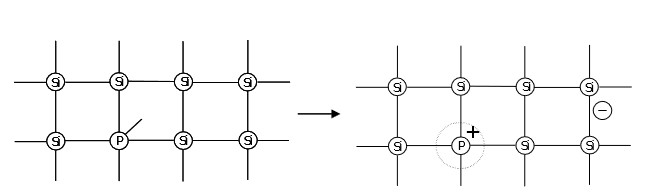
\includegraphics[width=\linewidth]{ndoping.jpg}
    \caption{n-doping (P)}
    \label{fig:ndoping}
\end{subfigure}
\begin{subfigure}{0.9\textwidth}
    \centering
    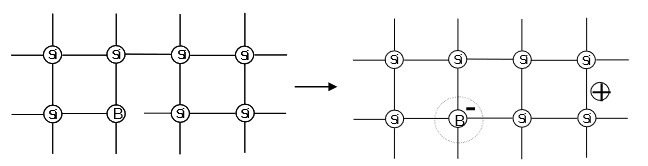
\includegraphics[width=\linewidth]{pdoping.jpg}
    \caption{p-doping (B)}
    \label{fig:pdoping}
\end{subfigure}
\caption{Doping in Si-crystals. The atom stays in both cases at its position \cite{instructions}.}
\end{figure}
In p-doping (see \cref{fig:pdoping}), an atom with fewer valence electrons than the base is used (e.g. Si as a base can be doped with B with 3 valence electrons). In this case, the missing electron is supplied by the lattice, leaving a freely movable hole. The now negatively charged ion stays at its place in the lattice.\\
The doping alters the Fermi-energy toward the conduction band. On the whole, however, the semiconductor stays electrically neutral.
\subsubsection{The p-n junction}\label{pnjunc}
Bringing a p-doped and n-doped semiconductor together forms a p-n-junction. In thermodynamic equilibrium, the holes and electrons diffuse into the respectively other due to the imbalance in concentration. In this process, they annihilate each other, leaving a area with few free charge carriers, the depletion layer (\cref{fig:depletion}.
\begin{figure}[H]
    \centering
    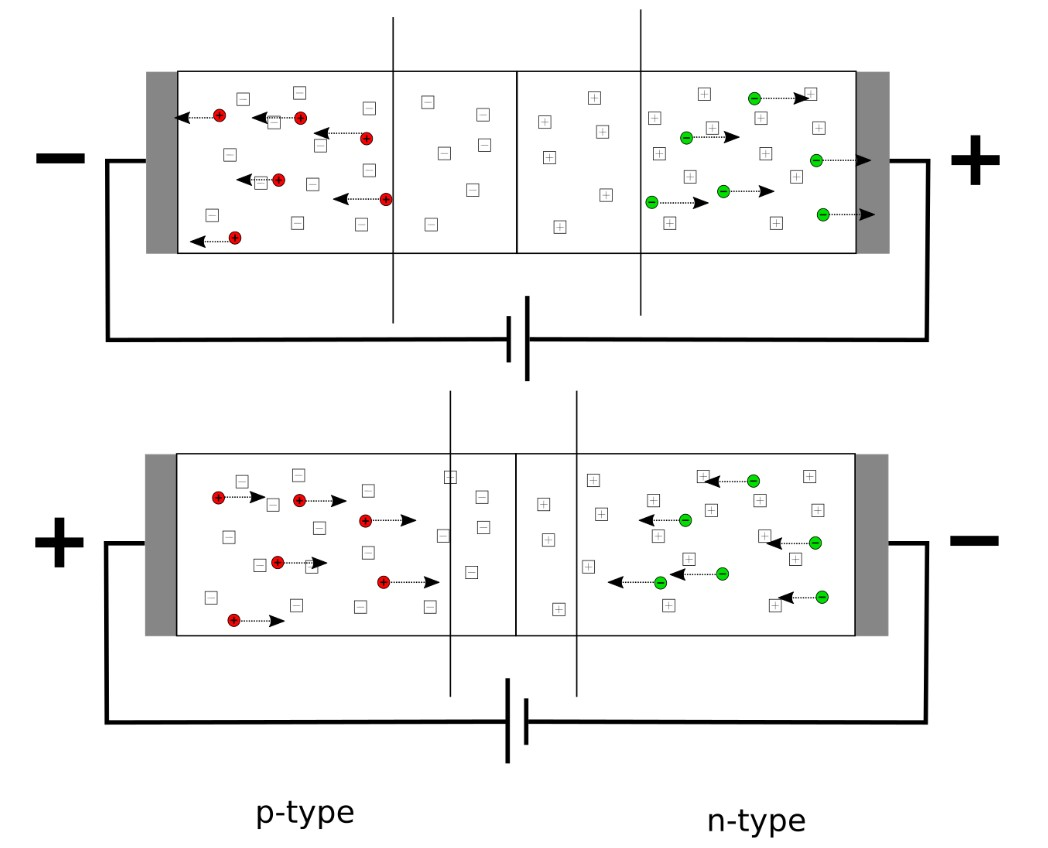
\includegraphics[width=0.7\linewidth]{depletion.jpg}
    \caption{Schematic of the p-n-junction with external voltage. The stationary bodies of the doping-atoms generate an electric field \cite{instructions}.}
    \label{fig:depletion}
\end{figure}
The bodies of the doping-atoms stay stationary however, creating a negatively charged region on the side of the p-semiconductor and a positively charged one on the side of the n-semiconductor, thus creating an electric field. At the same time, the charge creates a difference in potential, countering the diffusion, so that no current is measurable from the outside.
\paragraph{Diode-characteristics}
If one connects the junction to an external voltage with plus at the p-semiconductor and minus at the n-semiconductor, then free charge carriers are forced into the depletion layer from both sides (see the lower part of \cref{fig:depletion}), thus facilitating a current through this layer. \\
If one however switches the direction of the voltage, the charge carriers are pulled outward toward the contacts, thus enlarging the depletion layer and making the flow of current impossible (see the upper part of \cref{fig:depletion}). The p-n-junction is known as a diode in electrical engineering.\\ 
The characteristic curve of an ideal diode is described by the Shockley-equation
\begin{equation}
    I=I_S\cdot\left(\exp{e\frac{Ve}{nk_BT}}-1\right),\label{eq:shockley}
\end{equation}
with the outer voltage $V$, the saturation current $I_S$, the ideality factor $n$, the Boltzman-constant $k_B$ and the temperature $T$. $I_S$ is here dependent on the temperature and the width of the band gap $E_G$:
\[I_S\propto\exp{-\frac{E_G}{k_BT}}\]
\subsubsection{The illuminated p-n junction}
If the p-n-junction is illuminated, additional electron-hole pairs are created and the state of equilibrium of \cref{pnjunc} is disturbed. If the pair is created in the depletion layer, the electron is drawn toward the p-zone, while the hole is drawn toward the n-zone, where they create a potential at the outer edge of those zones. If one connects a consumer, a current, called photocurrent, runs through the cell and consumer. \\
If the pair is created outside the depletion layer, it is not affected by a force, until it is carried into the depletion layer via thermodynamic processes. An important influence on the effectiveness of solar cells is, that these pairs are not caught by impurities such as lattice defects before they reach the depletion layer.\\
One can characterize this process with an energy-level diagram such as in \cref{fig:energylevel}, where the cause of the force on the charge carriers is caused by the field of the depletion layer. This field is characterised by the voltage $V_D$, which can only be tapped outside the depletion layer as the open current voltage $V_{oc}$ if additional charge carriers get created by illumination of the p-n-junction. With higher illumination intensity, $V_{oc}$ rises, while the potential $V_D$ gets lowered, so that $V_{oc}$ approaches $V_D$, but never meets it. This can be explained by the diffusion current, which rises with more charge carriers being created, and pushes the electron-hole pairs back into the depletion layer, where they recombine. The diffusion current also rises with temperature, so that maximum efficiency can be achieved at low temperatures and high illumination intensities.
\begin{figure}[H]
    \centering
    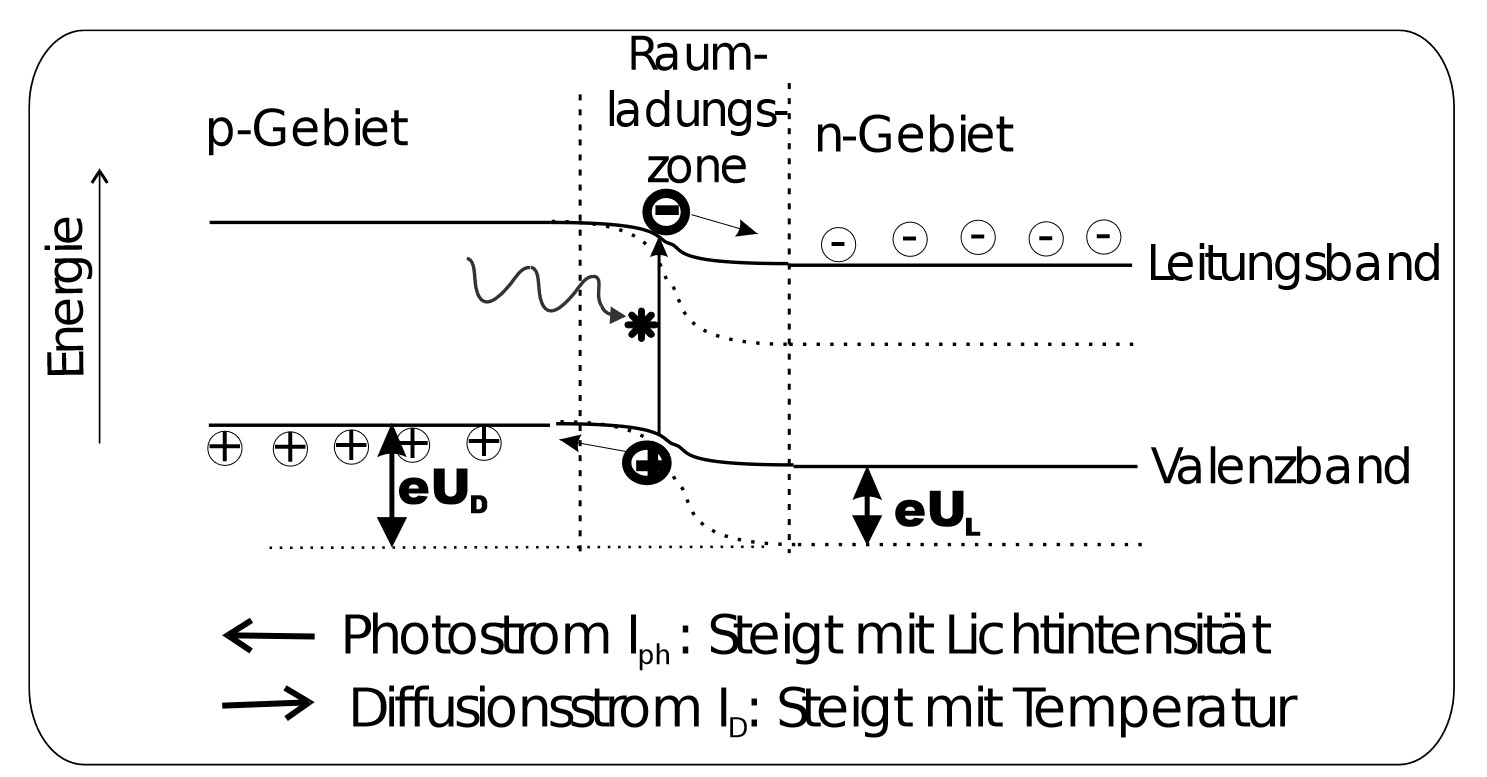
\includegraphics[width=0.8\linewidth]{energieschema.jpg}
    \caption{Energy-level-diagram. Electrons roll like stones downhill, holes rise like bubbles. Dotted lines are the situation without illumination, straight lines with illumination in an open circuit \cite{instructions}.}
    \label{fig:energylevel}
\end{figure}
\paragraph{Equivalent circuit of the solar cell}
The ideal solar cell can be viewed as a diode with an additional photocurrent $I_{ph}, I_{ph}<0$ and can thus be described by a Shockley-equation with the addition of $I_{ph}$:
\begin{equation}
    I=I_{ph}-I_S\cdot\left(\exp{e\frac{Ve}{nk_BT}}-1\right).
\end{equation}
A real cell however has losses, which can be characterised with parallel (representing e.g. leakage current) and series (e.g. bulk resistance) resistances $R_P$ and $R_S$ as in \cref{fig:circuit}, so that the total current of a real solar cell can be described as
\begin{equation}
    I_{ph}-I_S\cdot\left(\exp{e\frac{e(V_IR_S}{nk_BT}}-1\right)-\frac{V_IR_S}{R_P}.\label{eq:shockleymod}
\end{equation}
\begin{figure}[H]
    \centering
    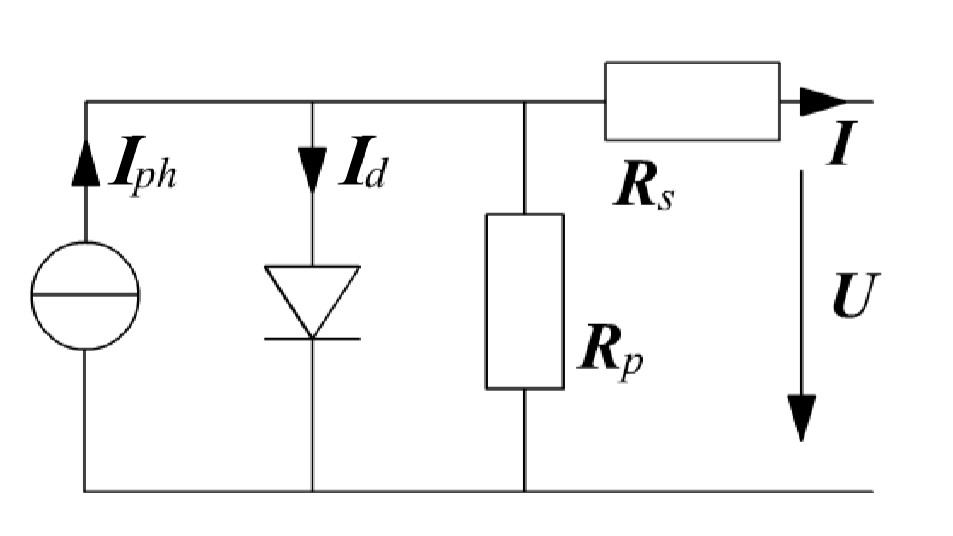
\includegraphics[width=0.6\linewidth]{circuit.jpg}
    \caption{Equivalent circuit of a real solar cell \cite{instructions}.}
    \label{fig:circuit}
\end{figure}
From \cref{eq:shockleymod} one can deduce that $R_S$ should be small and $R_P$ should be large.
\paragraph{I-V-curve of a solar cell}
The I-V-curve of a solar cell is displayed in \cref{fig:ivline}.
\begin{figure}[H]
    \centering
    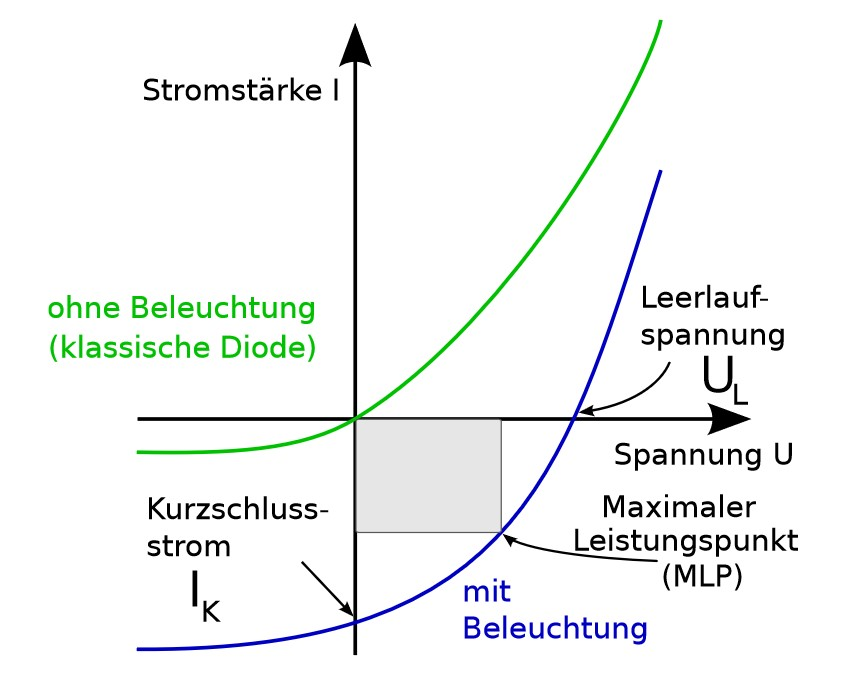
\includegraphics[width=0.9\linewidth]{ivline.jpg}
    \caption{I-V-curve with characteristic points \cite{instructions}. $I_K$ means $I_{sc}$, $U_L$ means $V_{oc}$, MLP means MPP. The green line is without illumination, the blue line with.}
    \label{fig:ivline}
\end{figure}
With the curve one determines the short circuit current $I_{sc}$, the open circuit voltage $V_{oc}$ and the maximum power point MPP where the power of the cell $P_{\text{MPP}}=V_{\text{MPP}}\cdot I_{\text{MPP}}$ is maximized. Another important parameter is the fullness-factor $FF=\dfrac{P_{\text{MPP}}}{I_{sc}\cdot V_{oc}}$. The efficency $\eta$ of the cell is can be calculated as
\begin{equation}
    \eta=\frac{|P_{\text{MPP}}|}{P_{\text{in}}}=\frac{FF\cdot|I_{sc}|\cdot V_{oc}}{P_{\text{in}}} \label{eq:eta}
\end{equation}
Thus, a large fullness-factor, short-circuit current and open-circuit voltage is desireable in a solar cell.
\subsubsection{Organic solar cells} 
Organic solar cells are differentiated from inorganic ones by virtue of them using organic materials, such as polymers, where the semiconducting properties are localized in the molecules, with a strong binding of the electron-hole pair to the molecule, which means that the pair is more properly an excitation of the molecule, called exciton. Thus, the mobility of electrons is far lower, necessitating the use of very thin sheets to still facilitate  the flow of current. This in turn necessitates a high absorption coefficient, which is given in many organic materials. The separation of the exciton happens via contact with another molecule that favours charge transfer, analogous to the p-n-junction. \\
As the exciton is however rarely created at a boundary, the exciton has to travel some distance. As its diffusion length is quite low ($<10\,$nm) and as it relaxes if it does not hit a boundary, the two materials are created in a mixed layer, with phase-separation in the order of magnitude of the diffusion length. The mixed layer however still has to have continuous paths of each materials to facilitate the transport of the charge carriers.
\section{Experimental setup}
For the experiment an "artificial sun" was used being an arrangement of 20 100W lamps aligned in an order that guarantees isotropic radiation on the experimental table. The light intensity could be adjusted manually. The light intensity was determined via a calibration diode.
\\
The inorganic cells are silicon cells from leXsolar.\\
For reproducable, empiric data, it was made sure to maintain the same heat for measurements (which did not always work very good), since the diode characteristic is heat-sensible, by adjusting the fans.\\
Furthermore the solar cells were always placed in the same spot. The hight of the experimental table was not altered.\\
For further measurements, different resistances, a load (fan), a thermometer and circuit elements were used.
\clearpage
\section{Procedure}\label{procedure}
\subsection{A: Diode-behaviour of a solar cell in darkness}\label{A}
The I-V-characteristic of a Si-solar cell was recorded in darkness (covered by a black cloth) and under one sun ($100\,\si{\frac{mA}{cm^2}}$) of incoming radiation. To achieve that value, a gauge-diode was placed at the same position as the solar cell. It is known that one sun of radiation would create a open circuit voltage of 32.2\,mV in the diode, and it was presumed that the relationship between voltage and radiation is linear. \\As in all other measurements, the voltage was increased in 100 equidistant steps from $-1\,$V to $1$\,V, with a waiting time at each step of 0.5\,s. The maximum current was limited to 1\,A. The result can be seen in \cref{fig:A}. The measurement was taken at 297\,K. One can clearly see the expected diode-behaviour in the unilluminated cell, blocking current until the breakthrough-voltage (here about 0.5\,V) is exceeded, at which point an electron-avalanche sets in, rapidly increasing current for small changes in voltage. 
\begin{figure}[H]
    \centering
    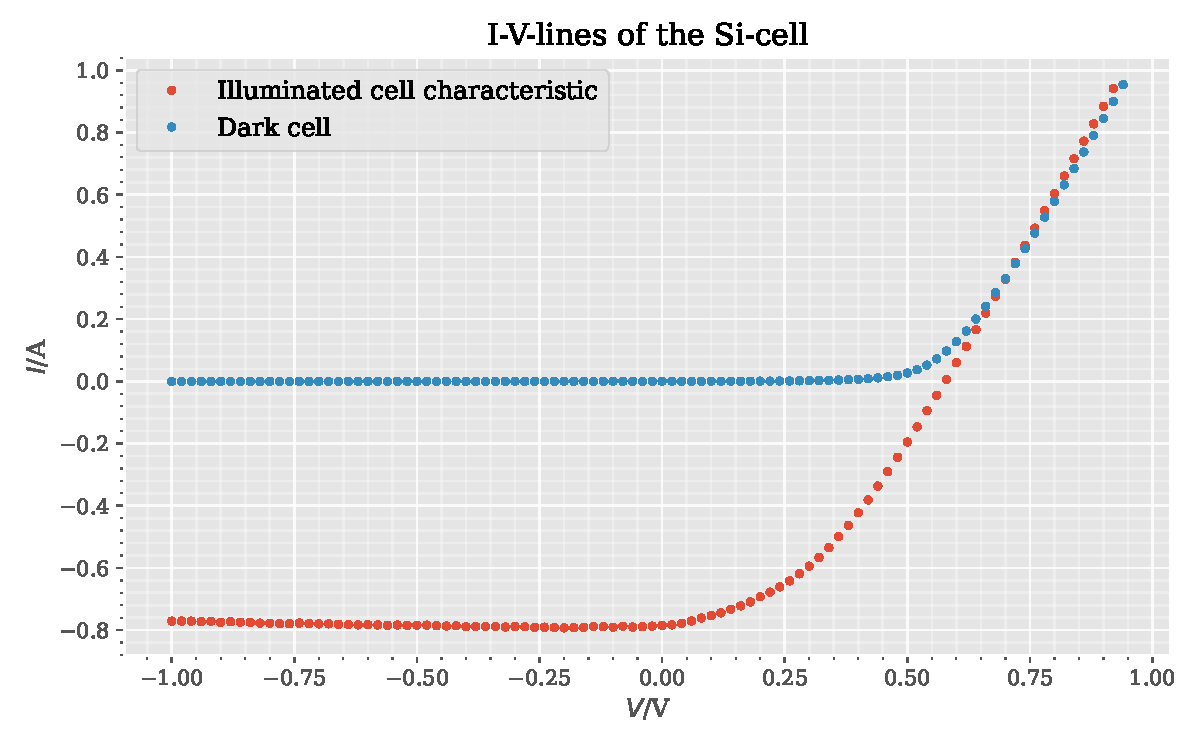
\includegraphics[width=\linewidth]{A.pdf}
    \caption{I-V-Characteristic of Si-cell}
    \label{fig:A}
\end{figure}
Due to the previous group exceeding the maximum current for the organic cell, it was unfortunately unavailable for measurement for us.\\
To determine the saturation current $I_S$, the ideality factor $n$ and the serial resistance $R_S$, a modified version of Shockley's Equation (\cref{eq:shockley}) for diodes with a series resistance is used:
\begin{align}
    I&=I_S\cdot\left(\exp{e\frac{V-IR_S}{nk_BT}}-1\right)\\
    \Rightarrow V&=n\frac{k_BT}{e}\ln{\frac{I+I_S}{I_S}}+IR_S\label{eq:vdepend}
\end{align}
To fit this equation, the instruction recommends to first determine $R_S$ via linear fit from the linear part of $U(I)$ (here $I>0.25$\,A and then use this value to plot $U^\prime=U-IR_S$ over the logarithm of the absolute current. $R_S$ then has to be varied to achieve a linear graph for large currents, which is then fitted logarithmically. The process can be seen in \cref{fig:A_fit}.\\
The first step returns 
\[R_S=0.39\,\Omega.\]
This is now used to plot $U^\prime=U-IR_S$, but $R_S$ has to be adjusted somewhat to achieve a linear tail, so that the final results from this method are:
\[R_S=0.31\,\Omega,\:
n=1.72,\:
I_S=\SI{4.10e-7}{A}
\]
It should be noted that these results are quite subjective, as the choice of $R_S$ is more or less free, and the choice of where to start fitting the logarithm is also not objective. Nevertheless, the so estimated parameters fit well within the expected values. $n$ is quite large, as usual values for it are fall between 1 and 2 \cite{pved}. The saturation current also lies within the typical range of \SIrange{10e-12}{10e-6}{A}.
\begin{figure}[H]
    \centering
    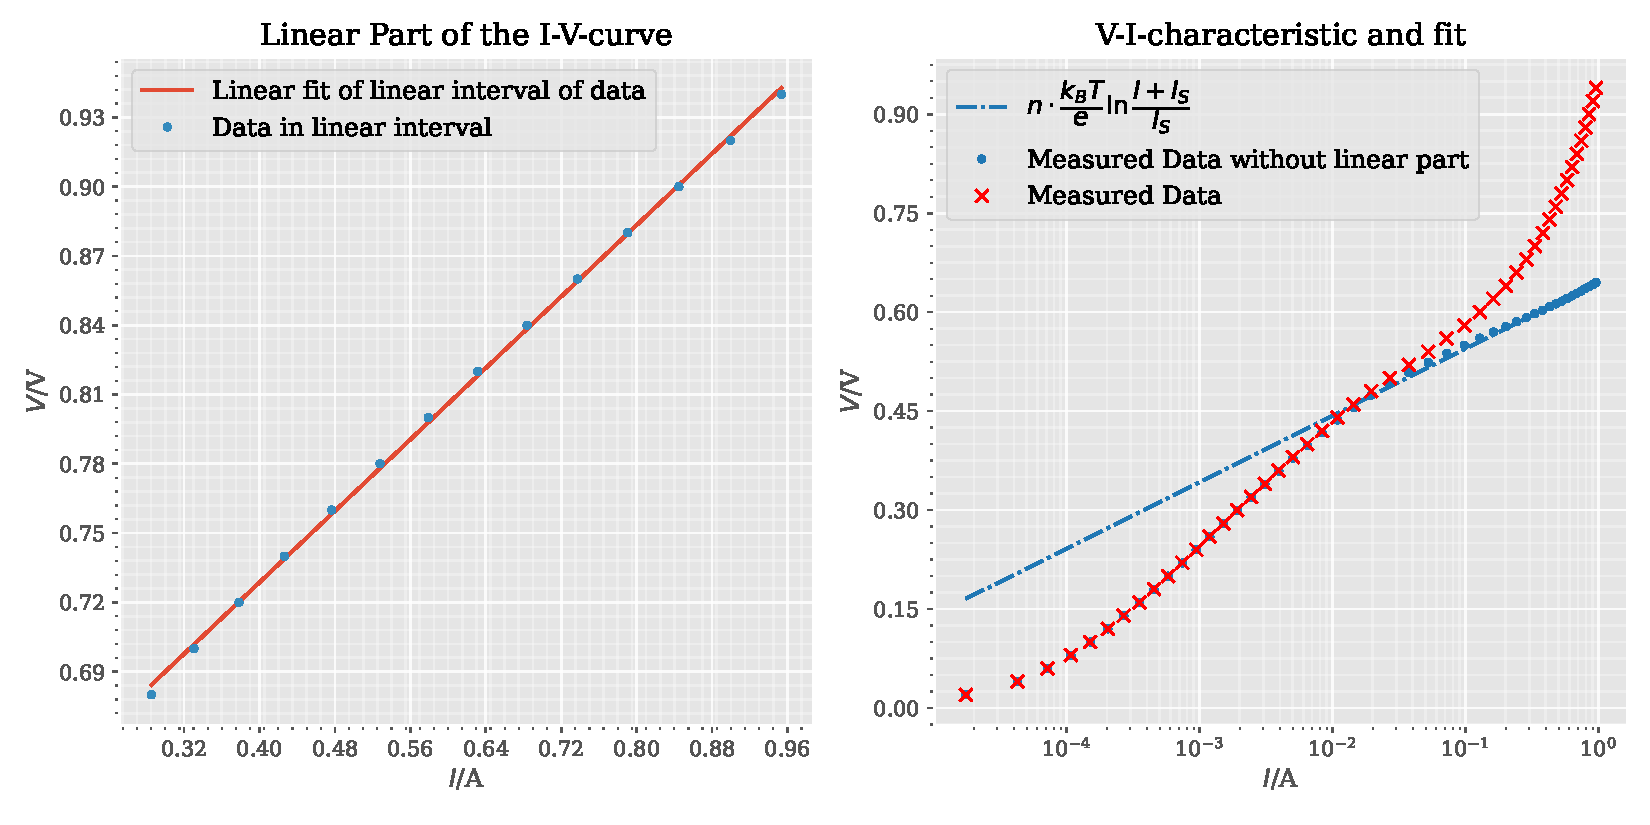
\includegraphics[width=\linewidth]{Afit.pdf}
    \caption{Fits of the V-I-curve of the dark cell.}
    \label{fig:A_fit}
\end{figure}
\subsection{B: The solar cell under illumination}
Next, the dependence of the cells characteristics on the illumination intensity were measured. The maximum illumination for this was chosen as the maximum achievable brightness, which corresponded to 37.1\,mV at the gauge diode. Then the light was dimmed to predetermined, logarithmically spaced values, as seen in \cref{tab:illumination}. The temperature varied in between measurements, as the fans could not keep up with the heat generation of the lamps. The temperatures are also noted in \cref{tab:illumination}. For the lowest value, the outer ring of lights had to be turned off, but as the illumination intensity was measured at the same position that the solar cell was at, this should not influence the results. Those can be seen in \cref{fig:B}, with black diamonds denoting the maximum power point. It has to be noted that too few measurements were taken to accurately pinpoint the MPP, as the difference between the values around it are very small. This might explain the unexpectedly low voltages of the MPP for low illumination intensities.\\
\begin{figure}[H]
    \centering
    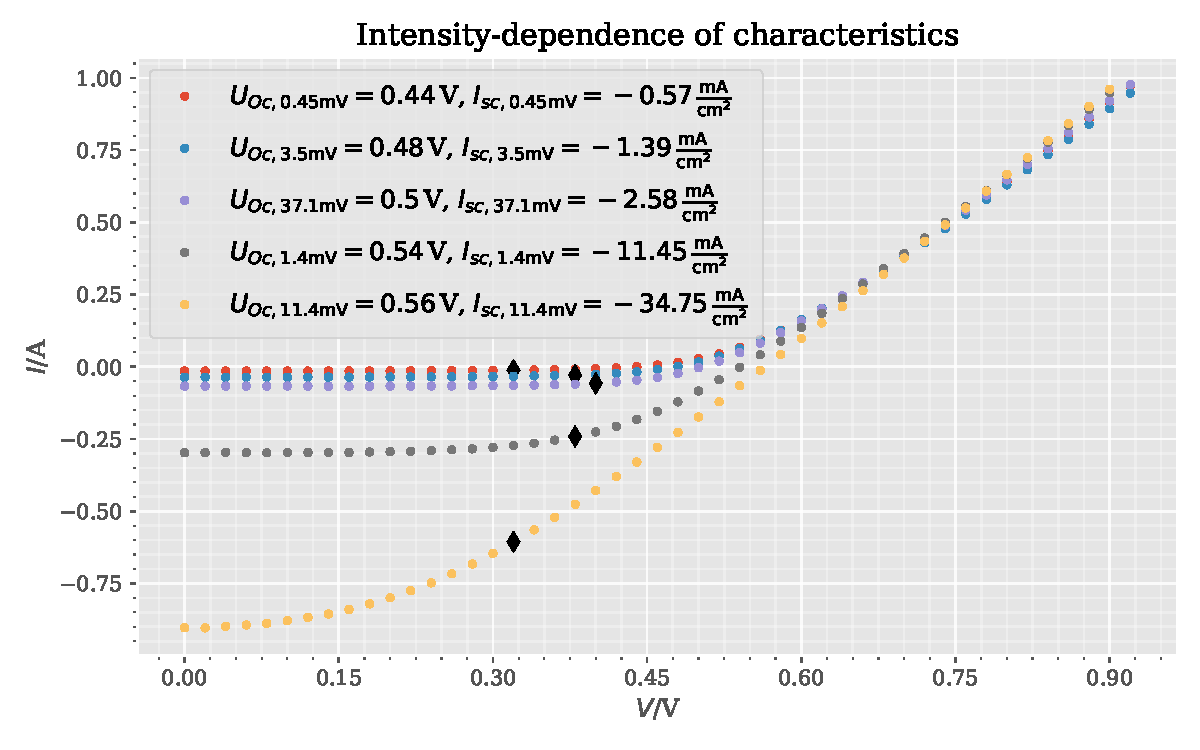
\includegraphics[width=\linewidth]{B.pdf}
    \caption{I-V-Characteristic of the same cell under different light intensities}
    \label{fig:B}
\end{figure}
At high voltages (greater than 0.6V) the curves all converge, resembling now a resistance. For low voltages, the short-circuit current decreases linearly, as can be seen in the lower part of \cref{fig:B_plot}. As in an ideal solar cell $j_{sc}=j_{ph}$, i.e. the short-circuit current conforms with the photocurrent, one can thus gather that the photocurrent is linearly dependent on the illumination. The open current voltage follows a logarithmic curve as can be seen in the upper plot of \cref{fig:B_plot}. The voltage should follow the dependence \cite{pved}
\[
V^\prime_{oc}=V{oc}+\frac{nk_BT}{e}\ln(P_{in}),
\]
so that from the fit parameters one can determine $V{oc}=0.621$\,V and $n=1.02$. The value of $n$ does not fit with the one determined in task A, however, the errors due to for example temperature fluctuations or calibration errors makes judgment over which $n$ is closer to correct very difficult.\\
\begin{figure}[H]
    \centering
    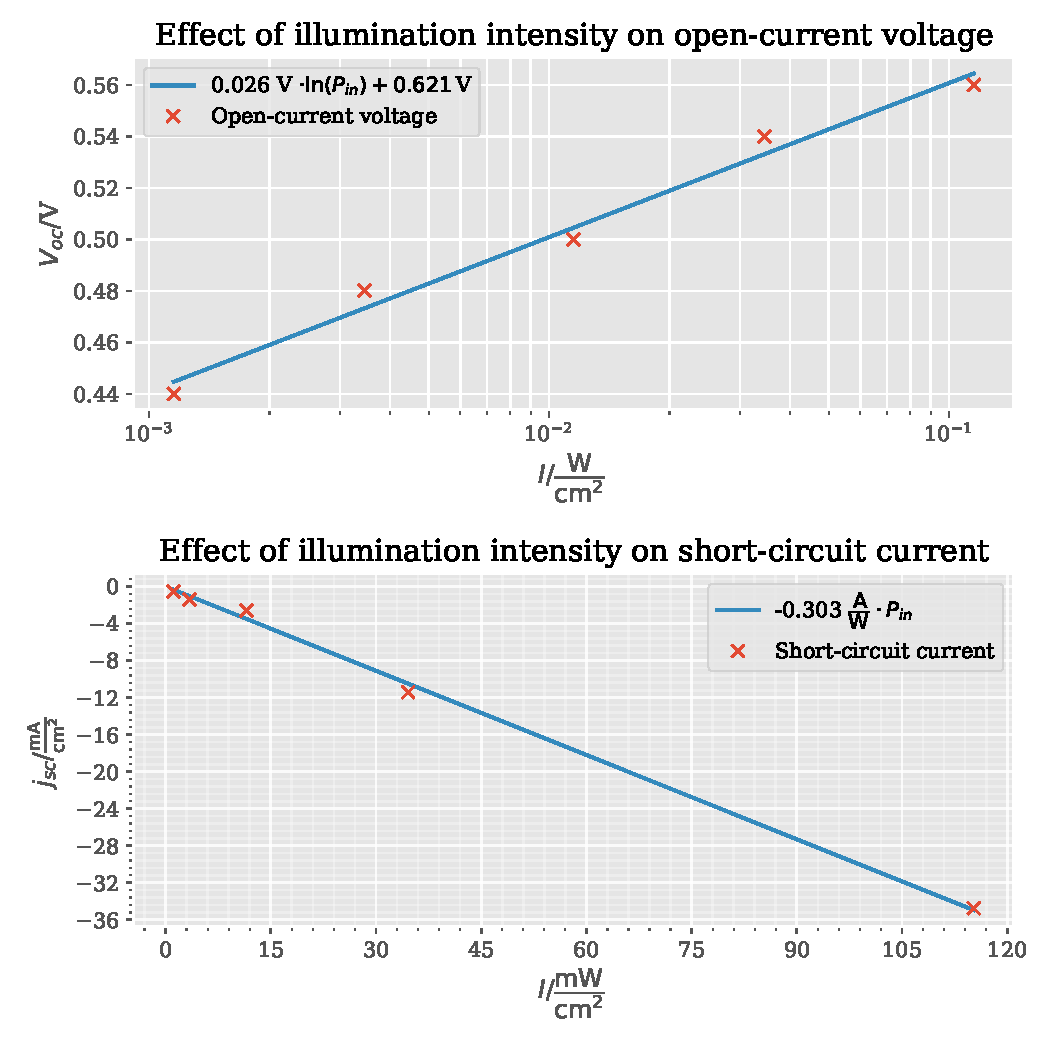
\includegraphics[width=\linewidth]{B_plot.pdf}
    \caption{Dependence of characteristic points on light intensity}
    \label{fig:B_plot}
\end{figure}
The fill-factor exhibits the expected behaviour of lowering toward either extreme, as the shunt resistance and the serial resistance respectively start degrading power-output.
\begin{table}[H]
\centering
    \caption{Characteristics of the solar cell at different light intensities}
\begin{tabular}{lrrrrr}
\toprule
{$P_\mathrm{in}$/mW} &  29.95   &  89.86   &  299.56  &  898.69  &  2995.65 \\
T / $^\circ$C & 31.1 & 32.7 & 36 & 39.8 & 45\\
\midrule
$\Vec{j}_{SC}/\si{\frac{mA}{cm^2}}$ &    -0.57 &    -1.39 &    -2.58 &   -11.44 &   -34.75 \\
$U_0$/V &     0.44 &     0.48 &     0.50 &     0.54 &     0.56 \\
$P_{MPP}$/mW &    -3.81 &   -11.08 &   -22.96 &   -91.74 &  -193.98 \\
FF &     0.59 &     0.64 &     0.68 &     0.57 &     0.38 \\
$\eta$ &     0.13&     0.12 &     0.08 &     0.10 &     0.06 \\
\bottomrule
\label{tab:illumination}
\end{tabular}
\end{table}

\subsection{C: Various experiments with solar modules}
For the following measurements, different wirings, shadings and amounts of solar panels are connected in order to investigate their influences on the output voltage. For all measurements in this part, the intensity was set to $I = \frac{1}{3}I_{sun}$ via the calibration diode.
\subsubsection{Different wiring}
First of all, 6 solar panels were connected in a way that maximizes $V_{OC}$ and $I_{SC}$ gently and  improves the efficiency $\eta$, visible in \cref{fig:modverschatt}. It was therefore decided to connect 2 panels each in a parallel manner and to connect those 3 pairs in series.\\
Now resistors were connected to the circuit, while examining especially the influence of the amount or resistance connected parallel and in series as can be seen in \cref{fig:C2}.\\
By looking at \cref{fig:circuit} and \cref{eq:vdepend} one can conclude that ideally, the series resistance should be minimized, reducing the current intensity of the solar cell, while the parallel resistance in order to prevent possible leakage currents should be maximized.\\
The I-V-characteristics with ($R_S, R_P$)-pairs shown in \cref{fig:C2} display this behaviour and the efficiency is maximized with this optimal wiring
, as can be seen in \cref{fig:modschaltungen} and \cref{tab:C2}.\\
In a real solar cell $R_S$ is created by inner resistance of the semi-conductor and the resistance of the contacts. $R_P$ is most likely created by impurities in the p-n-junction causing charges to flow in false directions.

\begin{figure}[H]\centering
  \begin{subfigure}[h!]{.3\textwidth}
    \begin{circuitikz} \draw
      (0,0) to[empty photodiode] (0,2)
      to[short] (2, 2)
      to[european resistor, l=$\SI{1}{\ohm}$] (2, 0)
      to[short] (0, 0);
      \draw (2,2)
      to[european resistor, l=$\SI{68}{\ohm}$] (4, 2)
      node[circ]{};
      \draw (2,0)
      to[short] (4, 0)
      node[circ]{};
    \end{circuitikz}
    \caption{Setup 1}
    \label{fig:schalt1}
  \end{subfigure}
  \begin{subfigure}[h!]{.3\textwidth}
    \begin{circuitikz} \draw
      (0,0) to[empty photodiode] (0,2)
      to[short] (2, 2)
      to[european resistor, l=$\SI{68}{\ohm}$] (2, 0)
      to[short] (0, 0);
      \draw (2,2)
      to[european resistor, l=$\SI{1}{\ohm}$] (4, 2)
      node[circ]{};
      \draw (2,0)
      to[short] (4, 0)
      node[circ]{};
    \end{circuitikz}
    \caption{Setup 2}
    \label{fig:schalt2}
  \end{subfigure}
  \begin{subfigure}[h!]{.3\textwidth}
    \begin{circuitikz} \draw
      (0,0) to[empty photodiode] (0,2)
      to[short] (2, 2)
      to[european resistor, l=$\SI{3.3}{\ohm}$] (2, 0)
      to[short] (0, 0);
      \draw (2,2)
      to[european resistor, l=$\SI{3.3}{\ohm}$] (4, 2)
      node[circ]{};
      \draw (2,0)
      to[short] (4, 0)
      node[circ]{};
    \end{circuitikz}
    \caption{Setup 3}
    \label{fig:schalt3}
  \end{subfigure}
  \caption{Different wirings of the solar module with differing resistances connected in series and parallel.}
  \label{fig:modschaltungen}
\end{figure}
\begin{figure}[H]
    \centering
    \includesvg[width=0.5\linewidth]{C1.svg}
    \caption{I-V-characteristic for a light curve for a module of 6 solar panels.}
    \label{fig:C1}
\end{figure}
\begin{table}[H]
\centering
    \caption{Characteristic parameters of the 6-panel-module.}
    \label{tab:C2}
\begin{tabular}{lrrrrr}
\toprule
$I_{SC} / \si{\ampere}$&$V_{OC} / \si{\volt}$&$P_{MPP}/ \si{\milli\watt}$&FF&$\eta$\\
\midrule
-0.5&1.6&-333&0.396&0.064\\
\bottomrule
\end{tabular}
\end{table}
\begin{figure}
    \centering
    \includesvg[width=0.5\linewidth]{C2.svg}
    \caption{Influence of different wirings on the MPP. Different setups are explained in \cref{fig:modschaltungen}. MPP-points are shown as black triangles.}
    \label{fig:C2}
\end{figure}
\begin{table}[H]
\centering
    \caption{Characteristic parameters of the solar module of 6 panels with different wirings according to \cref{fig:modschaltungen}.}
    \label{tab:C2}
\begin{tabular}{lrrrrr}
\toprule
&$I_{SC} / \si{\ampere}$&$V_{OC} / \si{\volt}$&$P_{MPP}/ \si{\milli\watt}$&FF&$\eta$\\
\midrule
Setup 1 &  -0.007&0.5&-1.0&0.26&0.0002\\
Setup 2 &  -0.359&1.6&-167&0.29&0.0321\\
Setup 3 &  -0.138&1.0&-35&0.24&0.0067\\
\bottomrule
\end{tabular}
\end{table}

\subsubsection{Different shadings}
In this measurement, the influence of the partial shadings of the solar module, still consisting of 6 panels is investigated, since for a real application, clouds etc. do alter the isotropic irradiation on the panels.\\
Therefore, 3 different setups are considered, as can be seen in \cref{fig:modverschatt}.\\
The I-V-characteristic light curves can be seen in \cref{fig:C3}. The shading was artificially done by putting a blanket on the panels. As one might expect, the absolute amount of $P_{MPP}$ is somewhat proportional to the shaded area, which is validated with the values shown in \cref{tab:C3}. 
% The geometrical amplification of area of the panels that is penetrated by radiation seems to also be a factor that at least the increase of current is dependent on (comparing setup b) and c)), but the absolute amount of area that is illuminated is the most influential on the efficiency. 
The massive drop in efficiency of the configurations in \cref{fig:schalt2} and \cref{fig:schatt3} come from the fact that the shaded parallel module acts as a significant series resistance, which massively cuts down the setups electrical viability, as in \cref{fig:schalt1}. To combat this, as cells can shut down in field conditions too, a parallel running free-wheeling diode is employed.
\begin{figure}[h!]\centering
  \begin{subfigure}[b]{.3\textwidth}\centering
    \begin{tikzpicture}[scale=.3]
      \draw[black, thick, fill=black] (0,0) rectangle (2,2);
      \draw (2,1) -- (3,1);
      \draw[black, thick, fill=black] (3,0) rectangle (5,2);
      \draw (2.5,1) -- (2.5,4);

      \draw[black, thick] (0,3) rectangle (2,5);
      \draw (2,4) -- (3,4);
      \draw[black, thick] (3,3) rectangle (5,5);
      \draw (2.5,4) -- (2.5,7);

      \draw[black, thick] (0,6) rectangle (2,8);
      \draw (2,7) -- (3,7);
      \draw[black, thick] (3,6) rectangle (5,8);
    \end{tikzpicture}
    \caption{Shading of the parallel cells.}
    \label{fig:schatt1}
  \end{subfigure}
  \begin{subfigure}[b]{.3\textwidth}\centering
    \begin{tikzpicture}[scale=.3]
      \draw[black, thick, fill=black] (0,0) rectangle (2,2);
      \draw (2,1) -- (3,1);
      \draw[black, thick] (3,0) rectangle (5,2);
      \draw (2.5,1) -- (2.5,4);

      \draw[black, thick, fill=black] (0,3) rectangle (2,5);
      \draw (2,4) -- (3,4);
      \draw[black, thick] (3,3) rectangle (5,5);
      \draw (2.5,4) -- (2.5,7);

      \draw[black, thick, fill=black] (0,6) rectangle (2,8);
      \draw (2,7) -- (3,7);
      \draw[black, thick] (3,6) rectangle (5,8);
    \end{tikzpicture}
    \caption{Shading of half of the module.}
    \label{fig:schatt2}
  \end{subfigure}
  \begin{subfigure}[b]{.3\textwidth}\centering
    \begin{tikzpicture}[scale=.3]
      \draw[black, thick, fill=black] (0,0) rectangle (2,2);
      \draw (2,1) -- (3,1);
      \draw[black, thick, fill=black] (3,0) rectangle (5,2);
      \draw (2.5,1) -- (2.5,4);

      \draw[black, thick, fill=black] (0,3) rectangle (2,5);
      \draw (2,4) -- (3,4);
      \draw[black, thick] (3,3) rectangle (5,5);
      \draw (2.5,4) -- (2.5,7);

      \draw[black, thick] (0,6) rectangle (2,8);
      \draw (2,7) -- (3,7);
      \draw[black, thick] (3,6) rectangle (5,8);
    \end{tikzpicture}
    \caption{Mix of setup (a) and (b).}
    \label{fig:schatt3}
  \end{subfigure}
  \caption{Different wiring-situations. Horizontal lines symbolise series connection, while vertical lines symbolise parallel connection.}
  \label{fig:modverschatt}
\end{figure}
\begin{figure}[H]
    \centering
    \includesvg[width=0.5\linewidth]{C3.svg}
    \caption{Influence of different shadings on the 6-panel-solar-module. The V-interval has been broadened, so that $V_{OC}$ is included. MPP-points are shown as black triangles.}
    \label{fig:C3}
\end{figure}
\begin{table}[H]

\centering
    \caption{Characteristic parameters of the solar module of 6 panels with different shadings according to \cref{fig:modverschatt}.}
    \label{tab:C3}
\begin{tabular}{lrrrrr}
\toprule
&$I_{SC} / \si{\ampere}$&$V_{OC} / \si{\volt}$&$P_{MPP}/ \si{\milli\watt}$&FF&$\eta$\\
\midrule
Setup (a) &  -0.0011&1.2&-0.5&0.37&0.0001 \\
Setup (b) &  -0.188&1.5&-130.5&0.46&0.0502 \\
Setup (c) &  -0.006&1.4&-4.9&0.60&0.0019\\
\bottomrule
\end{tabular}
\end{table}
\pagebreak
\subsubsection{Modified solar module}
Next up, a bigger module, consisting of 12 panels was considered. It turned out, that one panel was broken, so the measurements were done with a 11-panel-module.\\
The task was to make sure that the module provides a voltage of $V > \SI{12}{\volt}$. This could be achieved by connecting the panels in series. The light curves can be seen in \cref{fig:C4}. A load (fan) was connected to the circuit in order to obtain values for the working current and voltage (measuring with multimeter):
\begin{align*}
V_{W} &= \SI{5.2}{\volt} \\
I_{W} &=  \SI{137}{\milli \ampere}
\end{align*}
As one might imagine, the load decreases the efficiency (in this case by a factor of 2), while the short-circuit current is invariant and the open-circuit voltage increases slightly. This results in a smaller total amount of $P_{MPP}$ for the load circuit as can be expected and seen in \cref{tab:C4} by a factor of $\approx 2$.

\begin{figure}[H]
    \centering
    \includesvg[width=0.5\linewidth]{C4.svg}
    \caption{I-V-charateristics for a 11-panel-module. MPP-points are shown as black triangles. The V-interval has been broadened, so that $V_{OC}$ is included. Note that for the green plot, which describes the load connected to the circuit, there is an abrupt change in the current visible around $V \approx\SI{1.5}{\volt}$ and $V \approx\SI{1.7}{\volt}$. This is due to the fan turning on at these points, since a certain voltage is needed for it to run $\approx \SI{6}{\volt}$.}
    \label{fig:C4}
\end{figure}
\begin{table}[H]
\label{tab:C4}
\centering
    \caption{Light curve characteristic parameters of the solar module of 11 panels. Note that}
\begin{tabular}{lrrrrr}
\toprule
&$I_{SC} / \si{\ampere}$&$V_{OC} / \si{\volt}$&$P_{MPP}/ \si{\milli\watt}$&FF&$\eta$\\
\midrule
fan &   -0.24&5.1&-480&0.4&0.05 \\
Without fan & -0.24&5.9&-922&0.6&0.10 \\
\bottomrule
\end{tabular}
\end{table}
%\begin{table}[H]
%\centering
%    \caption{Dark curve characteristics of the solar module of 11 %panels}
%\begin{tabular}{lrrrrr}
%\toprule
%&$I_{SC} / \si{\ampere}$&$V_{OC} / \si{\volt}$&$P_{MPP}/ %\si{\milli\watt}$&FF&$\eta$\\
%\midrule
%fan &   -9.5e-06&0.16&-0.0004233&0.27812&4.44e-08
% \\
%Without fan &   -9.7e-06&0.18&-0.0004344&0.24786&4.5e-08\\
%\bottomrule
%\end{tabular}
%\end{table}

\subsection{D: Influence of the temperature}
In order to study the influence of the temperature on the open circuit voltage of an inorganic cell, $V_{OC}$ was measured for $ 30\si{\celsius}\le T \le 65\si{\celsius}$, while keeping the light intensity of one sun, as can be seen in \cref{fig:D1}. On top of that, the I-V-characteristics for the temperature extrema can be seen in \cref{fig:D2}.\\
As described in \cref{tab:D} it was quite difficult to measure $V_{OC}$ due to the rapidly changing temperature, induced by the lighting, even though the coolers were used to maintain the temperature at each level. Despite that, a linear relation can be nicely seen for $35 \si{\celsius}\le T \le 60\si{\celsius}$, which is a result of the equation of an ideal solar cell.\\
As can be seen in \cref{fig:D2}, the temperature does not have a big influence on the current, since the light intensity and thus the $e^-$-hole-pair-creation-rate doesn't change. 
\begin{figure}[H]
    \centering
    \includesvg[width=0.5\linewidth]{D.svg}
    \caption{Temperature dependence of $V_{OC}$.}
    \label{fig:D1}
\end{figure}
\begin{table}[H]
    \centering
    \caption{Measurement data for the temperature dependence experiment, where $\Delta \bar{T}$ is the assumed statistical measurement uncertainty due to the fact, that especially for the temperature extrema it was not possible to keep the temperature constant.}
    \begin{tabular}{c|c|c|c|c|c|c|c|c}
         $\bar{T} / \si{\celsius}$&30&35&40&45&50&55&60&65 \\ \hline
         $V_{OC} / \si{\milli\volt}$& 581&561&555&547&543&535&532&510 \\ \hline
         $\Delta \bar{T} / \si{\celsius}$&3&1&1&1&1&1&1&2
    \end{tabular}
    \label{tab:D}
\end{table}
Via \verb+curve_fit+ the T-V$_{OC}$-relation is approximated as a linear function, while excluding the measurement points for the temperature extrema, as can be seen in \cref{fig:D1}.\\
The obtained fit parameters are, while the measurement uncertainties are interpreted as statistical and result from the covariance-matrix of \verb+curve_fit+ as in all further fits:
\begin{align*}
\text{A} \pm \Delta \text{A}=&\,(1.29\pm0.06)\si{\milli\volt\per\celsius}\\
\text{B} \pm \Delta \text{B}=&\,(606\pm3)\si{\milli \volt}
\end{align*}
\begin{figure}[H]
    \centering
    \includesvg[width=0.5\linewidth]{D2.svg}
    \caption{I-V-characteristics for the temperature extrema.}
    \label{fig:D2}
\end{figure}

\pagebreak
\subsection{E: Behaviour under direct and diffuse irradiation}
For this part of the experiment, one inorganic solar cell was tilted in $10^{\circ}$-intervals and the short-circuit current was measured in dependence of the angle of the incoming light. The intensity for this measurement was again equal to one sun. The data in \cref{fig:E} sufficiently fits to a cosine-fit-function, while for the datapoints in the interval $30^{\circ}\le\Phi \le 70^{\circ}$ the difference between measurement and fit is relatively large. The relation to the cosine-function of the data can be explained by the fact that with decreasing degree between light source and solar cell, less and less photons hit the cell perpendicularly.\\
It is to be noted that the current is not vanishing at $\Phi=\SI{90}{^{\circ}}$, which is due diffuse radiation from other light sources, even though is was made sure that this was minimized by turning off all lights in the room and shutting down the blinds.
\begin{figure}[H]
    \centering
    \includesvg[width=0.5\linewidth]{E1.svg}
    \caption{Angular dependence of the current $I$.}
    \label{fig:E}
\end{figure}

\begin{table}[!htp]
    \centering
        \caption{Measurement data for the irradiation experiment. Notice, that for the second last measurement, the amperemeter heavily fluctuated, that's why an uncertainty ($\pm\SI{10}{\milli \ampere}$ is denoted there).}
    \begin{tabular}{c|c|c}
         $\Phi /^{\circ}$ & T/$\si{\celsius}$&I/$\si{\milli \ampere}$\\\hline \hline
         0&41.4&198\\
         10&42.5&196\\
         20&43.6&195\\
         30&45.6&192\\
         40&45.9&192\\
         50&45.8&187\\
         60&46.5&184\\
         70&38.4&176\\
         80&35.5&150$\pm10$\\
         90&34.4&124
    \end{tabular}
    \label{tab:Etemp}
\end{table}

One obtains the fit parameters as can be seen in \cref{fig:E}:
\begin{align*}
\text{A}=&\, 1.0 \\
\text{B}=& \,0.009\frac{1}{^{\circ}}
\end{align*}
\pagebreak
\section{Discussion}
The darkened cell clearly exhibits the properties of a diode. As stated in \cref{A}, the values determined for this diode fit well within the theoretically expected.\\
\begin{table}[H]
    \centering
    \begin{tabular}{c|c|c|c|c|c|c}
         $j_{sc}/\si{\frac{mA}{cm^2}}$&$V_{oc}/$V&$j_{\text{MPP}}/\si{\frac{mA}{cm^2}}$&$V_{\text{MPP}}/$V&$P$(MPP)/W&$FF$&$\eta$  \\\hline
        -30.19& 0.58 &-20.57  & 0.34& -0.18 & 0.40 & 0.07
    \end{tabular}
    \caption{Characteristic values of the Si-cell under one sun.}
    \label{tab:my_label}
\end{table}
\begin{table}[H]
    \centering
    \begin{tabular}{c|c|c}
         $R_S/\Omega$&$n$&$I_S$/A\\\hline
         0.31&1.72&$4.10\ten{-7}$
    \end{tabular}
    \caption{Characteristic values of the Si-cell as a diode.}
    \label{tab:my_label}
\end{table}
The listed $FF$ as well as $\eta$ are noticeably below the expected values of 0.7 and 0.2 respectively for typical Si cells (for example \cite{bsolar}). This may be explained by the fact that our solar cells are not made for commercial use and also quite battered from the frequent tests conducted with them. Also, at lower illumination strength a higher, more expected efficiency is achieved, which indicates that the cell was not designed to work at such high illumination strengths\\
As expected a small series resistance $R_S$ and a large parallel resistance $R_P$ are optimal for a real circuit (see \cref{tab:C2}). \\
It was shown that the temperature dependence of $V_{OC}$ is linear, which is a result of diffusion, caused by increased thermal movement inside the p-n junction working against the photocurrent.\\
The results of the different shadings experiment in \cref{tab:C2} show that it has a non-neglectible effect on the efficiency of solar cells and has to be compensated in real circuits for realistic applications.\\
The last experiment showed that the light incidence angle has a big influence on the generated current. In general the position of solar-cell-modules (tilting, distance to light source) and their shading are important parameters that contribute to their efficiency and the generated current.\\
The determined value for the resistance of the cell as a diode is also low, with more typical values being  \SIrange{1}{25}{\ohm}. The order of magnitude is however still reasonable. The behaviour under different illumination intensities is mostly as expected, even if the drop off at high illumination is somewhat extreme. \\
These results would be more meaningful if an error could have been determined. To do this, however, multiple measurements per voltage would have had to be taken, which the instructed settings (and the given time) did not permit. 

\printbibliography


\end{document}
